\documentclass[]{sigchi}
% Use this command to override the default ACM copyright statement
% (e.g. for preprints).  Consult the conference website for the
% camera-ready copyright statement.

%% HOW TO OVERRIDE THE DEFAULT COPYRIGHT STRIP --
%% Please note you need to make sure the copy for your specific
%% license is used here!
% \toappear{
% Permission to make digital or hard copies of all or part of this work
% for personal or classroom use is granted without fee provided that
% copies are not made or distributed for profit or commercial advantage
% and that copies bear this notice and the full citation on the first
% page. Copyrights for components of this work owned by others than ACM
% must be honored. Abstracting with credit is permitted. To copy
% otherwise, or republish, to post on servers or to redistribute to
% lists, requires prior specific permission and/or a fee. Request
% permissions from \href{mailto:Permissions@acm.org}{Permissions@acm.org}. \\
% \emph{CHI '16},  May 07--12, 2016, San Jose, CA, USA \\
% ACM xxx-x-xxxx-xxxx-x/xx/xx\ldots \$15.00 \\
% DOI: \url{http://dx.doi.org/xx.xxxx/xxxxxxx.xxxxxxx}
% }
\toappear{}

% Arabic page numbers for submission.  Remove this line to eliminate
% page numbers for the camera ready copy
% \pagenumbering{arabic}

% Load basic packages
\usepackage{balance}       % to better equalize the last page
\usepackage{graphics}      % for EPS, load graphicx instead 
\usepackage[T1]{fontenc}   % for umlauts and other diaeresis
\usepackage{txfonts}
\usepackage{mathptmx}
\usepackage[pdflang={en-US},pdftex]{hyperref}
\usepackage{color}
\usepackage{booktabs}
\usepackage{textcomp}
\usepackage{nameref}

\usepackage[backend=biber, style=numeric, sorting=nty, firstinits=true, url=false]{biblatex}
%\usepackage{custom}

\addbibresource{paper.bib}


% Some optional stuff you might like/need.
\usepackage{microtype}        % Improved Tracking and Kerning
% \usepackage[all]{hypcap}    % Fixes bug in hyperref caption linking
\usepackage{ccicons}          % Cite your images correctly!
% \usepackage[utf8]{inputenc} % for a UTF8 editor only

% If you want to use todo notes, marginpars etc. during creation of
% your draft document, you have to enable the "chi_draft" option for
% the document class. To do this, change the very first line to:
% "\documentclass[chi_draft]{sigchi}". You can then place todo notes
% by using the "\todo{...}"  command. Make sure to disable the draft
% option again before submitting your final document.
\usepackage{todonotes}

% Paper metadata (use plain text, for PDF inclusion and later
% re-using, if desired).  Use \emtpyauthor when submitting for review
% so you remain anonymous.
\def\plaintitle{Why did they win?\\Visualizing NBA teams across multiple seasons}
\def\plainauthor[#1]{#1}
\def\plainauthors[#1]#2#3{#1, #2, #3}
\def\emptyauthor{}
\def\plainkeywords{Information Visualization; CHI; NBA}
\def\plaingeneralterms{}

% llt: Define a global style for URLs, rather that the default one
\makeatletter
\def\url@leostyle{%
  \@ifundefined{selectfont}{
    \def\UrlFont{\sf}
  }{
    \def\UrlFont{\small\bf\ttfamily}
  }}
\makeatother
\urlstyle{leo}

% To make various LaTeX processors do the right thing with page size.
\def\pprw{8.5in}
\def\pprh{11in}
\special{papersize=\pprw,\pprh}
\setlength{\paperwidth}{\pprw}
\setlength{\paperheight}{\pprh}
\setlength{\pdfpagewidth}{\pprw}
\setlength{\pdfpageheight}{\pprh}

% Make sure hyperref comes last of your loaded packages, to give it a
% fighting chance of not being over-written, since its job is to
% redefine many LaTeX commands.
\definecolor{linkColor}{RGB}{6,125,233}
\hypersetup{%
  pdftitle={\plaintitle},
% Use \plainauthor for final version.
  pdfauthor={\plainauthors[Yannick Boesmans]{Yannick Laevaert}{Yves Langeraert}},
%  pdfauthor={\emptyauthor},
  pdfkeywords={\plainkeywords},
  pdfdisplaydoctitle=true, % For Accessibility
  bookmarksnumbered,
  pdfstartview={FitH},
  colorlinks,
  citecolor=black,
  filecolor=black,
  linkcolor=black,
  urlcolor=linkColor,
  breaklinks=true,
  hypertexnames=false
}

\pagenumbering{arabic}

% create a shortcut to typeset table headings
% \newcommand\tabhead[1]{\small\textbf{#1}}

% End of preamble. Here it comes the document.
\begin{document}

\title{\plaintitle}

\numberofauthors{3}
\author{%
  \alignauthor{\plainauthor[Yannick Boesmans]\\
    \affaddr{KU Leuven}\\
    \email{yannick.boesmans}\\
    \email{@student.kuleuven.be}}\\
  \alignauthor{\plainauthor[Yannick Laevaert]\\
    \affaddr{KU Leuven}\\
    \email{yannick.laevaert}\\
    \email{@student.kuleuven.be}}\\
  \alignauthor{\plainauthor[Yves Langeraert]\\
    \affaddr{KU Leuven}\\
    \email{yves.langeraert}\\
    \email{@student.kuleuven.be}}\\
}

\maketitle

\begin{abstract}
    Visualization of sports data is very common in recent years as access to
    data has increased. The abundance of data and audience allows for new and
    innovative presentations. In this paper we describe an interactive
    visualization of the NBA competition over the last 30 years. With three
    different views, we allow the user to explore data about NBA seasons
    including standings, team statistics, transfers and player statistics. The
    d3.js framework was used to develop this visualization. 
\end{abstract}

%TODO keywords
\category{H.5.m.}{Information Interfaces and Presentation
  (e.g. HCI)}{Miscellaneous} \category{}{}{}

\keywords{\plainkeywords}

\section{Introduction}

The National Basketball Association (NBA) is the most famous professional
basketball league in the world\cite{nbawiki}. As in every other sports
branch, a lot of data and statistics about players, teams, games and seasons
are available, mainly in large tables. Despite the large amount of data
available, gathering useful insights from this data can be surprisingly
challenging. In our work we try to present this data in an innovative but still
intuitive way, allowing the user to draw meaningful conclusions.

In the \nameref{sec:goal} section we describe the goal of the visualization and the
target audience. In the \nameref{sec:data} section, we describe the data used, including its origins, advantages and limitations. The \nameref{sec:literature} section gives an overview of related literature and web resources, including related
visualizations. This includes both visualizations of NBA or other sports data,
as well as visualizations tackling an issue encountered during the development of
our visualization. In the \nameref{sec:visualization} section, the visualization itself is described. We give an overview of the different stages of development
of the visualization, as well as the major design decisions.
The \nameref{sec:lessonslearned} section describes some interesting lessons we have learned from the project and in the \nameref{sec:futurework} section we discuss potential  improvements of the final visualization. We conclude in the  
\nameref{sec:conclusion} section. Appendix~\ref{sec:terminology} contains definitions 
for common basketball terms used in this paper.

\section{Goal and Target Audience}\label{sec:goal} 
The visualization's goal can be best summarized by the following sentence:
``Why did a certain team win the NBA Championship?'' The visualization focuses
on exposing relations between team performance and their player roster over
several years. It allows users to find explanations for major improvements and
declines in team performance.  The visualization allows exploration of NBA data
by lay persons.  More specifically, the visualization does not focus on premade
explanations for phenomenons visible in the NBA data. By providing easy and
intuitive access to the data, the visualization allows users to draw their own
conclusions. The visualization's target audience are lay persons. Specifically,
basketball fans are the core of our target audience. It can be of particular
interest with the recent surge in fantasy leagues, for which data analysis is
paramount to a player's success~\cite{fantasy,fantasyskill}.

\section{Data}\label{sec:data}
The data visualized is a subset of the data available on basketball statistics
site basketball-reference\cite{basketball-reference}. It is a wide range of data including common basketball performance statistics, such as field goals, percentage of shots scored, shooting distance, minutes played per season, number of personal fouls made, salaries and much more . All of this data is available as time-series. These statistics are available for each player individually for each season. Aggregated data for entire teams and for entire seasons is also available. Additionally, individual game statistics are also available, including playoff games. In our visualization we only use data from 1984 onwards. This is done because of rule changes in the NBA which changed the number of teams competing and the
competition's structure. To simplify implementation of our visualization, only
data after the last major rule change was used.  The data we use includes league
standings and playoff rankings for each team, team overall statistics, the
team's roster and individual player statistics for each year, including the
PER~(Player Efficiency Rating)\cite{per}. 

The data was gathered by scraping the basketball-reference site using the
provided download capabilities. Most of the data was downloaded in csv format,
while some tables had to be manually scraped. This process was automated using
Python scripts. The data was then combined in a preprocessing step. In this
step, each team's playoff rankings were calculated based on the matches played
during the playoffs, and the rest of the data was combined into json format. The
final preprocessing step combined all data into one json file. A model of the
available data can be seen on figure~\ref{fig:data}.

\begin{figure}
\centering
  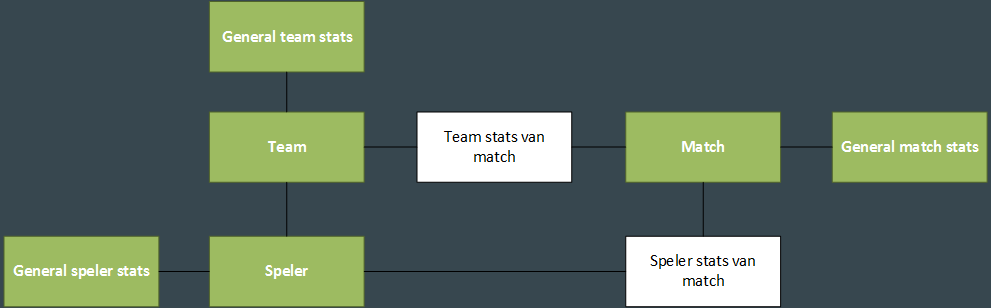
\includegraphics[width=1.0\columnwidth]{figures/data}
  \caption{An overview of the data.}
  \label{fig:data}
\end{figure}

\section{Related Work}\label{sec:literature}
Recently, there has been an increase in the interest in visualizations of sports
data. This is best exemplified by the workshop on sports data visualization at
the IEEE Visualization Conference in 2013\cite{ieeevis}. 

There are a number of traditional basketball visualizations. One of the most
popular ones is the shot chart. This visualizes the shots made by a player or team. Different methods can be used, going from a scatterplot to hexagonal charts where the shots are grouped into hexagonal regions, to a heatmap. This is often done for the the area in and around the three-point line, but it can als be done for the whole attack side of the field, as seen in the Vorped visualisation\cite{vorped}. Because shots of the own side only happen rarely, it's not shown in shot charts. Shot chart provides insight into the shooting ability of a
player\cite{goldsberry,stephenchu}.

This view features heavily in Peter Beshai's Buckets\cite{peterbeshai}. This is
an extensive visualization of NBA player data. It provides not only the player's
shot chart for various years, but his shooting signature and several line graphs
as well. It is strongly focused on individual player's shooting abilities. 

Visualizations focusing on basketball teams and their performance are
significantly more difficult to find. For the playoffs, there is the traditional
playoffs bracket~\cite{tournamentladder}. This bracket structure has the
advantage of being well known and as such, not requiring much explanation. It is
flawed however. It duplicates much information by displaying teams multiple
times. 

An interesting alternative is the sunburst tournament
visualization\cite{sunburst}. As the name suggests, this visualizes the
tournament as a sunburst, with the winning team taking the part of the circle
closer to the center. This does not eliminate the problem of the recurring teams
however.

For the wimbledon tennis tournament, an enclosed circles visualization was
created~\cite{enclosedcircles}. This visualization eliminates the repeating
occurrences of the same team. However, it wastes a lot of space. 

England's Permier League results were visualized by Ami Sedghi for the
Guardian\cite{premierleague}. This visualization shows the team's rankings as
line graphs and allows highlighting of individual teams.

Tan et al. created an adaption of the traditional tournament bracket to better
support moden interaction\cite{adaptivitree}. The tool, AdaptiviTree, changes
the brackets shape and adds colored lines to show available information as the
user picks his own bracket.

An alternative to the traditional bracket structure can be found in the
visualization of the race to the white house in 2012 made for the New York Times
by Mike Bostock and Shan Carter\cite{whitehousepath}. They use a tree-like
structure where each split represents a state being one by one candidate or the
other. The interactivity is very important here as it allows users to highlight
one possible path out of many.

The entire history of the NBA and the best teams were analyzed by
fivethirtyeight~\cite{fivethirtyeight}. They calculated an ELO-score\cite{elorating} 
for all teams an visualized them on line graphs. 

In the article written by Johannes Becker\cite{nbaempires}, the Simple Rating System 
score (SRS score) is used to compare teams over the last 40 seasons in the NBA. The 
SRS score is represented by a color hue. For comparing quantative values, this is 
not the most ideal characteristic to use as explained by John Mackinglay\cite{automatingdesign}. Nevertheless, some interesting findings are found and presented. By giving a green stroke to the rectangle of the champion of a season, 
it's easy to see which teams have won the NBA championship frequently. This way 
they have divided the last 40 seasons in three eras being the Los Angeles Lakers 
versus the Boston Celtics era, the Michael Jordan era and the Tim Duncan era. 

Pagno et al. provide a number of different visualizations\cite{starplots}. The
most interesting one is the starplot. This plot several statistics for a team on
an axis pointing radially outward from a common center. These points are then
connected. It allows the user to get basic information about a team or player at
a glance. Because of this speed of conveying information, it is also a prevalent
visualization in sports games.


%Related work/References

%Shot charts
%http://peterbeshai.com/buckets/app
%http://vorped.com/1-nba/2015-2016/player/6667/emmanuel-mudiay/
%https://github.com/amatlin/NBAvis
%https://thedatagame.com.au/2015/09/27/how-to-create-nba-shot-charts-in-r/
%http://savvastjortjoglou.com/nba-shot-sharts.html?utm_source=Python+Weekly+Newsletter&utm_campaign=5185ff0538-Python_Weekly_Issue_202_July_30_2015&utm_medium=email&utm_term=0_9e26887fc5-5185ff0538-312727397
%http://toddwschneider.com/posts/ballr-interactive-nba-shot-charts-with-r-and-shiny/

%Standings
%https://source.opennews.org/en-US/articles/nyts-512-paths-white-house/
%http://projects.fivethirtyeight.com/complete-history-of-the-nba/#warriors
%http://www.theguardian.com/news/datablog/interactive/2013/jun/03/premier-league-season-visualised
%http://gizmodo.com/5927503/all-the-major-sport-competitions-since-1903-condensed-in-beautiful-circular-graphics
%http://www.nbaplayoffsbracket.com/2016/index.php
%http://nyloncalculus.com/2015/08/07/as-nba-empires-rise-and-fall/
%http://inf.ufrgs.br/~lsguedes/skooth/Publications_&_Works_files/nbavis_final.pdf
%http://research.microsoft.com/pubs/64282/tvcg2007-adaptivitree.pdf
%http://www.student.kuleuven.be/~s0217391/mume/deliverables/paper.pdf

%Other
%https://graphics.stanford.edu/wikis/cs448b-10-fall/FP-RuthEric-HeddlestonKate?action=AttachFile&do=get&target=448bPaper.pdf
%http://www.scribblelive.com/blog/2014/03/20/the-power-of-sports-data-visualizing-passes-between-nba-players-offers-new-game-insights/
%http://lemonchiu.github.io/NBA-Visualization/


\section{Visualization}\label{sec:visualization}
The visualization consists of three parts:
\begin{itemize}
    \item The play-off view: a compact view on the play-offs per season
    \item The statistics (zoom) view: a more detailed view on a statistic of a
        selected team
    \item The team view: a detailed view on how good or bad a team scores on a
        specific field position
\end{itemize}

The technique used, follows the standards of information visualization. It provides
an overview, allows zooming and filtering and provides details on
demand\cite{mantra,multipleviews,automatingdesign}. The play-off view provides
the full overview which allows filtering by team. The statistics view provides
the ability to zoom into one specific team. There some details are provided
instantly, while others can be procured by hovering over certain elements.

All three views are discussed in more detail below. The three views are
available to the user on a single webpage, where they are organized in a 
vertical layout with fixed scrolling. Navigation with the keyboard is 
supported as well. The user start on the play-off view and is able to 
navigate to the statistics and team views by scrolling down or clicking 
on teams. A different season can be selected with the left and right
arrows or by clicking on the timeline. The timeline is a fixed part of the
visualization. It is visible in the three different views. Navigation 
with the keyboard for switching between the three different views is 
supported as well.

We did not opt for the traditional minimalistic approach used in information 
visualizations. The data-ink design principles were kept in mind, but we also 
focused on aesthetics instead of maximizing the data-ink ratio. So the choice 
was made to use a thematic background. This was done to improve the 
attractiveness of the visualisation on the one hand and the users' memory of 
it on the other hand\cite{aesthetics}. 

\begin{figure}
\centering
  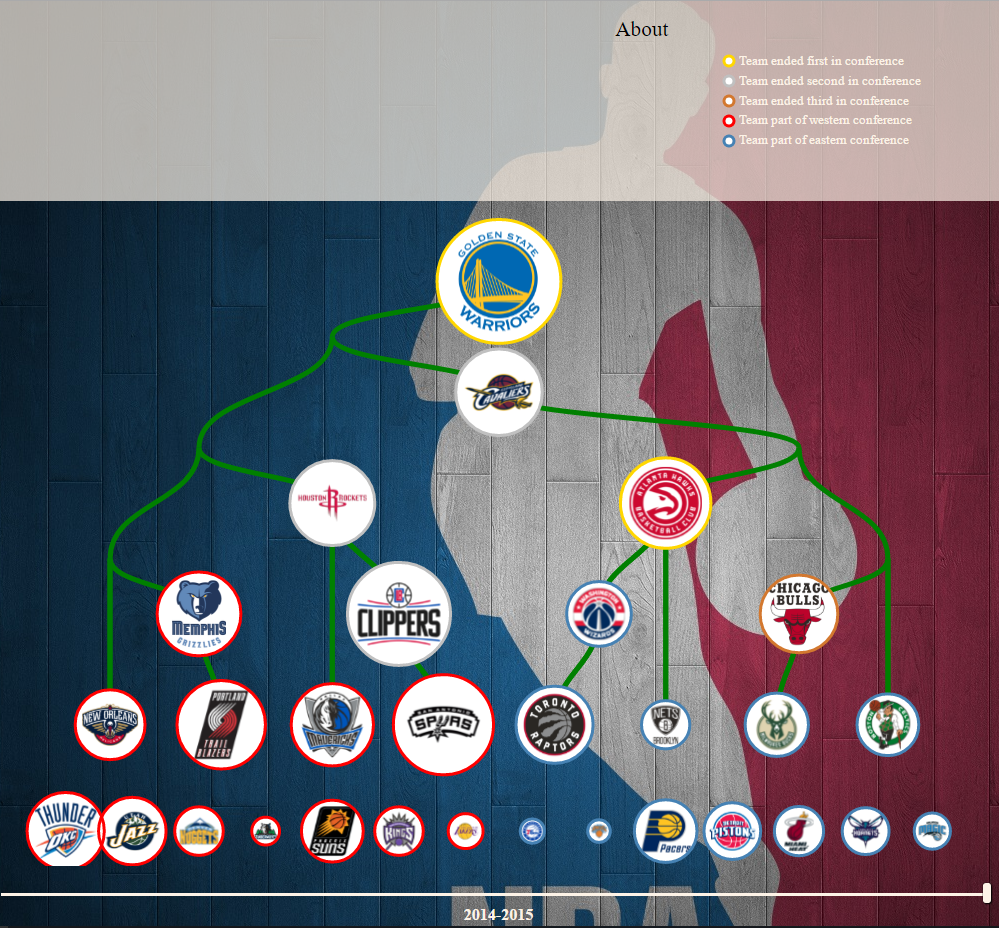
\includegraphics[width=1.0\columnwidth]{figures/playoffviewwithcontext}
  \caption{The play-off view without a team selected.}~\label{fig:playoffviewnoteam}
\end{figure}

\begin{figure}
\centering
  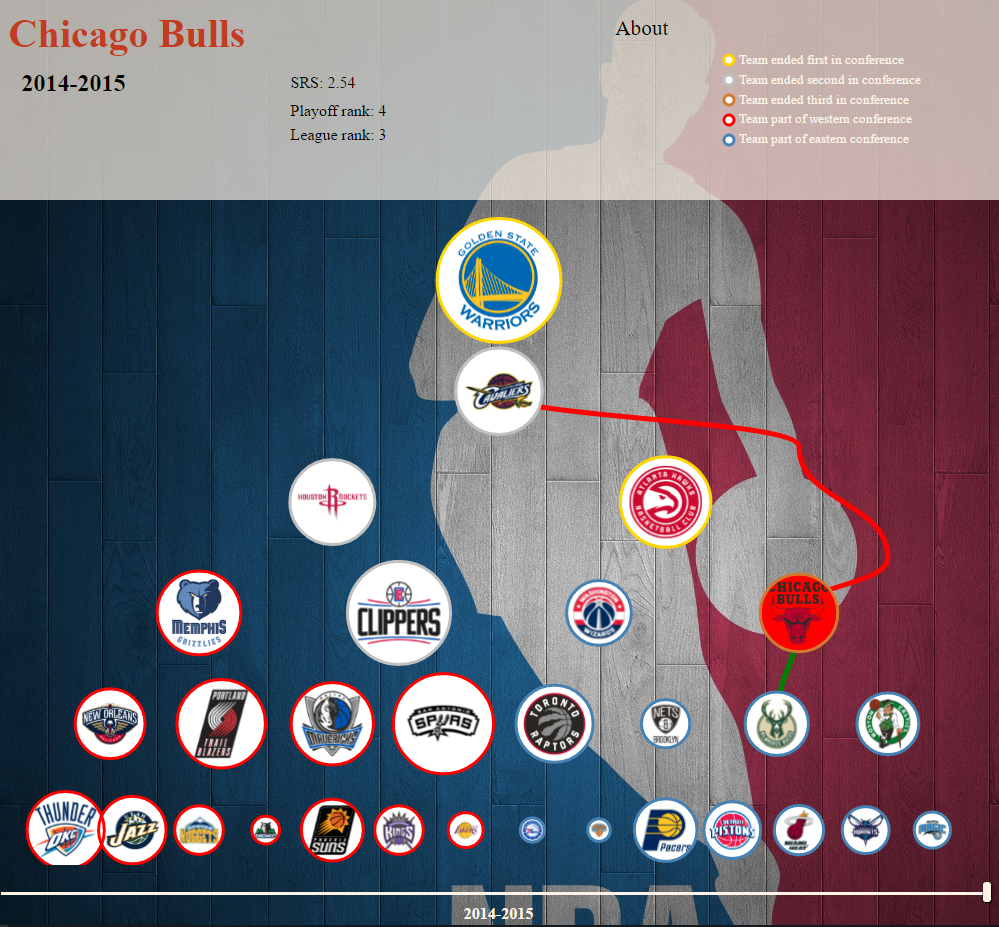
\includegraphics[width=1.0\columnwidth]{figures/playoffviewteamselected}
  \caption{The play-off view with a team selected.}~\label{fig:playoffviewteam}
\end{figure}

\subsection{The play-off view}
This view informs the user of the roster and end positions in the NBA play-offs
for a selected season, in general or for a selected team. The play-off view is 
shown in figure~\ref{fig:playoffviewwithcontext}.The view consists of
two parts: 
\begin{itemize}
    \item Context section: the top part informs the user about the selected team
    and shows a legend of the play-off view.
    \item Bubble section: this section represents the play-offs of the selected
    season.
\end{itemize}

\subsubsection{Context section}
The context section contains a legend for the bubble section. The bubble's
borders are gold, silver or bronze if the team ended respectively first, second
or third in the regular competition. Teams that didn't end on a podium place
during the regular competition have a red or blue stroke color indicating the
team's region, respectively the western or eastern conference. The context
section also contains a link to the ``About'' page where the user can get an
explanation of the visualization with its different views, can get some
background information about the NBA and the terminolgy used, and can check the
source of the data used in the visualization. If the user hovers over or selects 
a team in the bubble section, the context section shows more information about that 
team, as shown in Figure~\ref{fig:playoffviewteamselected}. The information shown 
includes the SRS score, the end position in the play-offs and the end position in 
the regular competition.

\subsubsection{Bubble section}
This section presents the roster and end positions of the play-offs for a
selected season. Every team is respresented by a circle with the logo of the
team inside it. The size of the circle represents the SRS score using an own
interpretation of perceptual scaling because the (Flannery) Appearance
Compensation is not usable with a domain of both negative and positive values.
An exponential function with exponent 1.5 was used. This way the proportion
between the area of a bigger and the area of a smaller circle will be greater
than the proportion of values the areas represent.

The curved lines between teams represent the fact that those teams have 
encountered each other in the playoffs. Each row represents an end position 
in the play-offs. The higher a team is, the further it has come.  From the 
top to the bottom the rows represent the winner of the final (rank 1), loser 
of the final (rank 2), losers of the semi-finals (rank 3), losers of the 
quarter-finals (rank 4), losers of the eighth finals (rank 5). The last row 
represents the teams that did not make it to the play-offs (rank 6). 

This simple presentation intuitively puts the winning teams higher than the
losing teams. The winner and loser of a certain game can be easily derived from 
their relative vertical position. It is also clear that for a team to be on a 
higher level, the team needs to have played and won a series of matches against 
one other team at every level below them~\ref{fig:playoffviewteamselected}. 
This view is further reinforced by highlighting a team and its matches and 
opponents when hovering over it. Additional team information is then also shown 
in the context part.

%\begin{figure}
%\centering
%  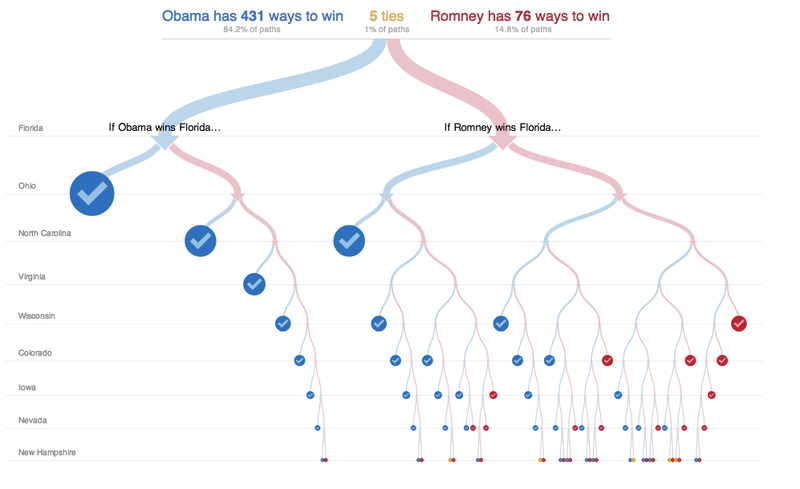
\includegraphics[width=1.0\columnwidth]{figures/presidentcandidatesvisualization}
%  \caption{The path of president candidates in their road to become president.}~%\label{fig:whitehousepath}
%\end{figure}

\begin{figure}
\centering
  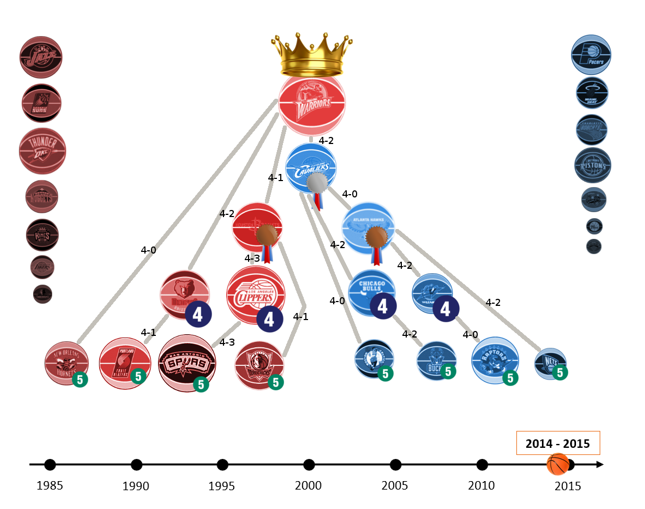
\includegraphics[width=1.0\columnwidth]{figures/playoffviewfirstdesign}
  \caption{First design of the play-off view.}~\label{fig:firstdesignplayoffview}
\end{figure}

\begin{figure}
\centering
%  \missingfigure{}
  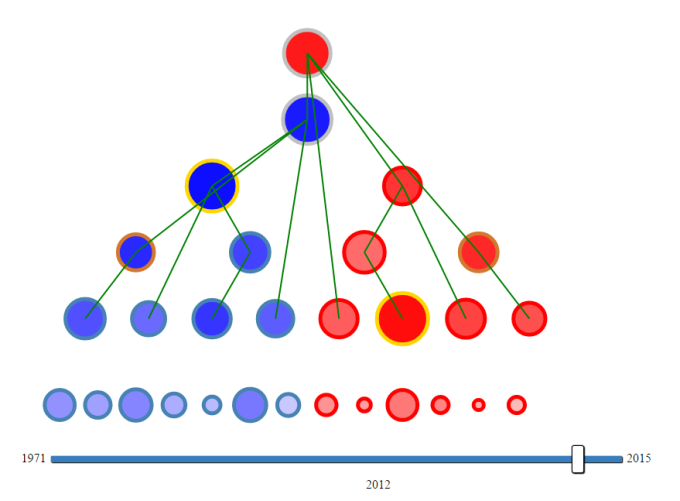
\includegraphics[width=0.9\columnwidth]{figures/playoffviewfirstimplemantation}
  \caption{First implementation of the play-off view.}~\label{fig:firstimplementationplayoffview}
\end{figure}


\subsubsection{Previous designs}
Our initial design used the team circles' lightness to indicate their final
ranking in their region. The hue was used to show the league they were part of.
According to the Ranking of Perceptual Tasks~\cite{automatingdesign} this is a
good property for ordered values like the regular competition ranking. But the
combination of the logo's of the teams with the colors resulted in an overload
of information and made it more difficult to compare the end ranking of
different teams. 

As an alternative we tried the same view without the logo's. It turned out this 
was inconvenient because you could not instantly see which team is represented 
by which circle. Therefore we've chosen to only use the teams' logos.

Our initial play-off view was too dense because of the connections between teams
as well. Teams that played against each other were connected directly. When
searching for alternatives to reflect on our choice we discovered a similar
visualization in a totally different context\cite{whitehousepath} as explained in 
the section \ref{sec:literature}. With the idea of this visualization in mind, our 
visualization gives a cleaner view of the competitors for a specific team compared 
to our original sketch. Hence we decided to adapt our visualization. We added an 
intermediate connection point between two teams to more clearly indicate how teams competed to 
become the NBA champion.

%\todo{Hierarchy = sorting = facilitate trends of winners
%position have a meaning in the play-off view
%when selecting circle => zoom/more detail
%Bubble principle of 
%- Symmetry (whole = play-off)
%- conectedness arc = games played
%Pre attentive characteristics
%- size of circles
%- hue to highligt selections or indicate increase decline arrows next view}

We initially also considered a map view to show the teams and their regular
competition ranking on a map of the USA. However, this view had no additional
value compared to the play-off view except for the geographical position, which
has no importance for our visualisation. Furthermore we've found a visualisation
of the NBA with a map view~\cite{mapviewvisualization} similar to our idea, so
we decided to not implement this map view. 

\begin{figure}
\centering
  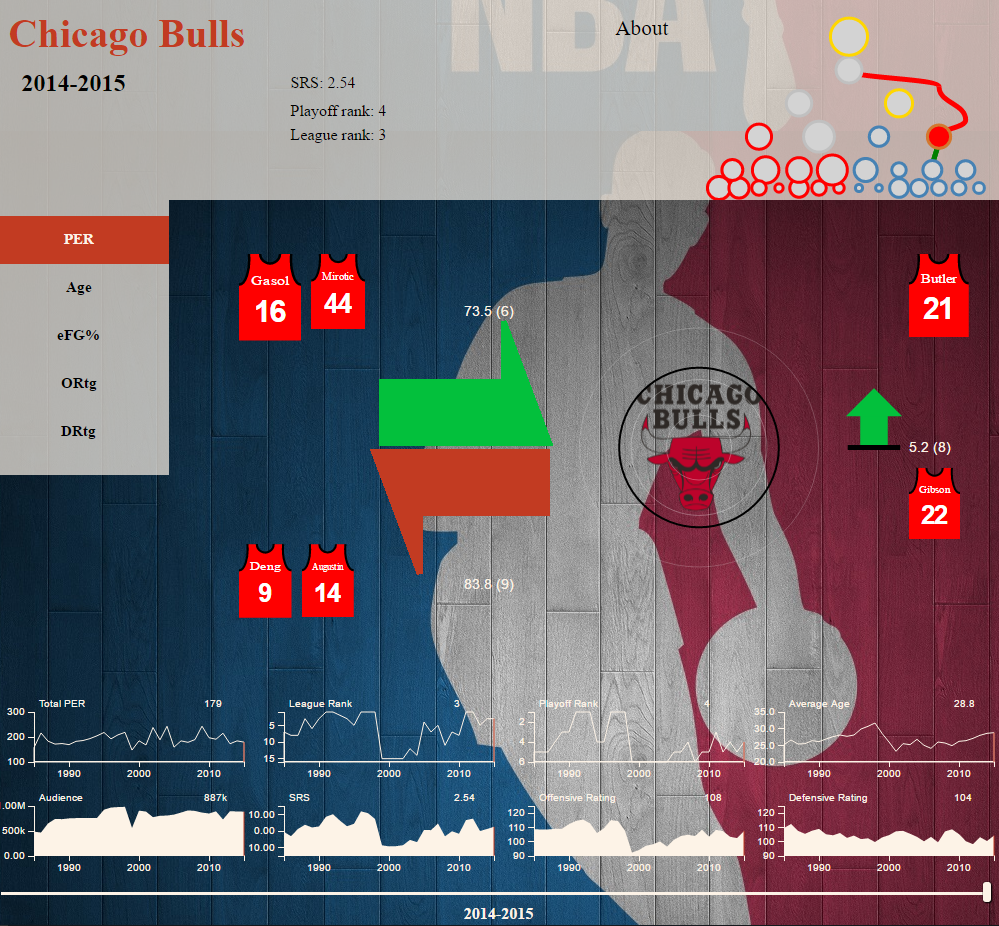
\includegraphics[width=1.0\columnwidth]{figures/statisticsview}
  \caption{The statistics view.}~\label{fig:statisticsview}
\end{figure}

\subsection{The statistics view}
The statistics view gives a user a clear overview of how a statistic has been
influenced in the selected season compared to the season before. The statistics
view is showed in Figure~\ref{fig:statisticsview}. The view consists of 3
coordinated parts:
\begin{itemize}
    \item Context section: the top part informs the user of the context of the
        selected team
    \item Arrow section: this section illustrates why a statistic has changed
        compared to the previous season
    \item Selected statistics section: team statistics and how they evolve over
        time
\end{itemize}

\subsubsection{Context section}
The context section is partly identical to that of the play-offs view. The
team's information is also displayed in the top left. In the top right, the
bubble section of the play-offs view is displayed in a reduced, minimalistic
form. This view is repeated to create a sense of continuity between the
different views and provide context of the current position in the
visualization. The team shown in the statistics view is highlighted on this
smaller bubble section as well. Replicating this section also alleviates
short-term memory issues. It prevents the need to scroll back and forth between
the different views constantly. 

\subsubsection{Arrow section}
This section illustrates a change for a chosen statistic for the selected team in 
the selected season compared to the previous season. This gives a user more 
insight into why a statistic changed over time and how this change has affected 
team performance. The selected team is represented by a circle in the same way as 
explained in the play-off view. To give the user a better interpretation of the SRS 
value of the circle, three other reference circles are drawn. These are 
transparant with a lightgrey border. They show the maximum, average and minimum SRS 
value of the NBA in the selected season. The change for the chosen statistic is 
represented by three arrows:
\begin{itemize}
    \item Arrow on the left pointing towards the circle: indicating the
        influence of players who joined the team.
    \item Arrow on the right of the circle: indicating how the team internally
        changed, e.g. by training its players
    \item Arrow on the left pointing away from the circle: indicating the
        influence of players who left the team 
\end{itemize}
The value of the change in statistic is shown next to the arrow. The number of 
players responsible for the change is shown between brackets. Their are shown 
jerseys next to the arrows as well. These are the jerseys of the two players that 
had the biggest contribution to the influence represented by that arrow.  
On the left, there is a possibility to chose a statistic. The possibilities 
are the PER value, the age, the effective field goal percentage, the offensive rating 
and the defensive rating. Below this, player information is shown when a user hovers
over a player's jersey. 

\subsubsection{Selected statistics section}
Below the arrow section, multiple line and area charts show how the selected 
team has performed over the years. The different statistics shown are the 
total PER of the whole team, the league rank, the playoff rank, the average age 
of the team, the audience, the SRS-value of the team, the offensive rating and 
the defensive rating of the team. A user interacts with the visualization by 
shifting the bar indicating the current year displayed or the timeline. By 
doing this the view gets updated and the user can see the impact on the team 
in the context section and why the statistic changes in the arrow section. 
These charts enable the user to identify peaks or drops in a certain statistic. 
By interacting with the visualization, previous seasons can be inspected to try 
to find explanations or following seasons can be inspected to see if a team 
responds in a specific way or what the consequences are. This view provides 
a lot of additional information to users by allowing them to see correlations 
between statistics and phenomena quickly and easily.

\subsubsection{Previous designs}
This view has not changed much compared to the initial design. The only difference 
was the position of the arrow and jerseys for the players who stayed, which were 
originally in the team circle, and so the logo was not showed. 
The design of the arrows did not change. The incoming and outgoing 
arrows are maybe more intuitevly than the arrow for the stayed players, but we did 
not find any alternatives we could use.

\begin{figure}
\centering
  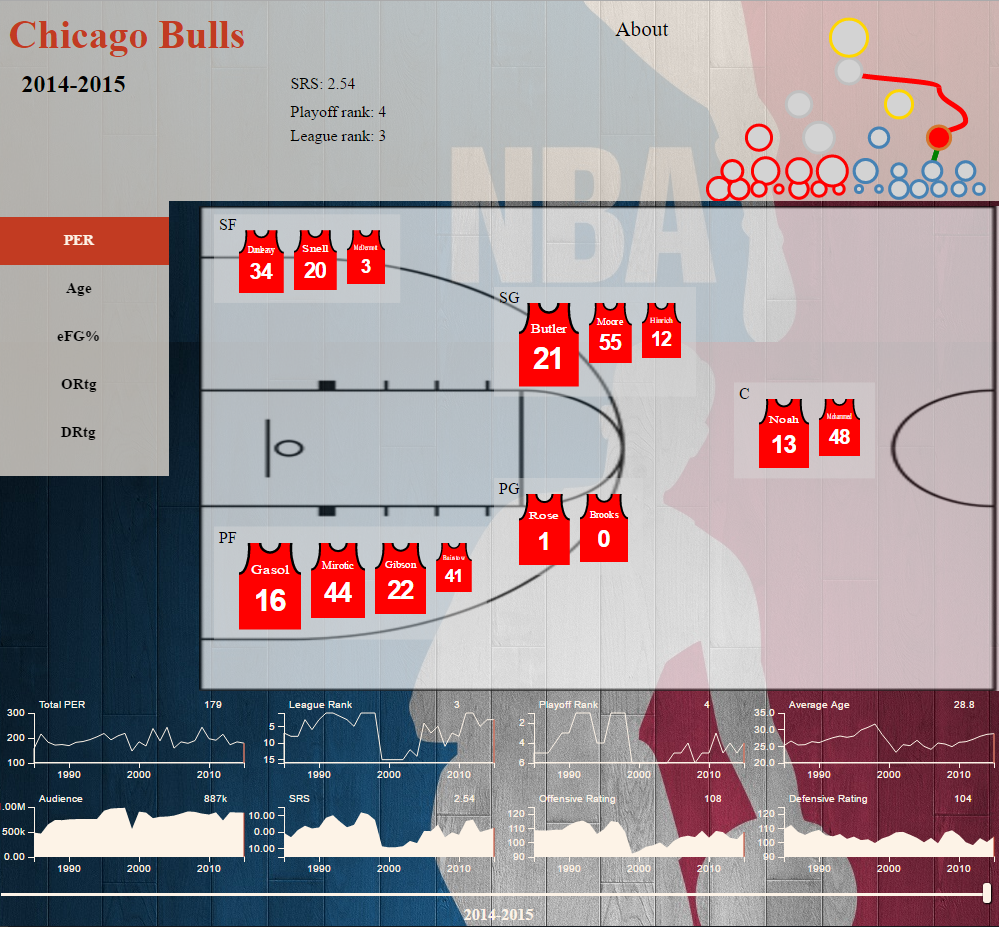
\includegraphics[width=1.0\columnwidth]{figures/teamview}
  \caption{The team view.}
  \label{fig:teamview}
\end{figure}

\subsection{The team view}
The team view gives a user a detailed view on the strength of the team on the 
different field positions. The team view is showed in Figure~\ref{fig:teamview}. 
The view consists of 3 coordinated parts:
\begin{itemize}
    \item Context section: the top part informs the user of the context of the
        selected team
    \item Field section: this section illustrates why a statistic has changed
        compared to the previous season
    \item Selected statistics section: team statistics and how they evolve over
        time
\end{itemize}
The context section and the selected statistics section are fixed parts in the 
statistics and team view, and are therefore not explained again for this view.

\subsubsection{Field section}
This view shows each player of the team on its field positions. Players are
represented by their jerseys. Jerseys aligned next to each other share the same
position, which is indicated as well. The size of a jersey illustrates a
players performance according to the chosen statistic. The possible statistics 
are shown on the left and are the same as those in the arrow section of the 
statistics view. As well as the statistics view, this view should give the user 
the ability to search for explanations why a team is performing better or worse 
over seasons. On the other hand, a user can see what impact a change in team 
characteristics has on its overall performance. This view should give a user 
insight on how strong or weak a particular team is for a specific field position. 
A user can then scroll through time to see how field positions evolve and what 
the influence is over time.

\subsubsection{Previous designs}
Initially we designed this view more elaborate. When the user would click on a
jersey, specific player information would be shown together with a number of
player statistics in the form of small multiples. A bell curve should have
informed how a player scores compared to his team, other players in the league
on his position or all other players in the league. We considered other charts
for the small multiples as well. A box plot or bullet was less clear for us to
indicate where a player stands compared to the group he was compared with. This
part of the visualization was not our main focus. Because of the lesser
importance and because of time and resource constraints, it has not been fully
developed. A sketch including the small multiples view on the bottom right is
shown on Figure~\ref{fig:smallmultsketch}.

\begin{figure}
\centering
  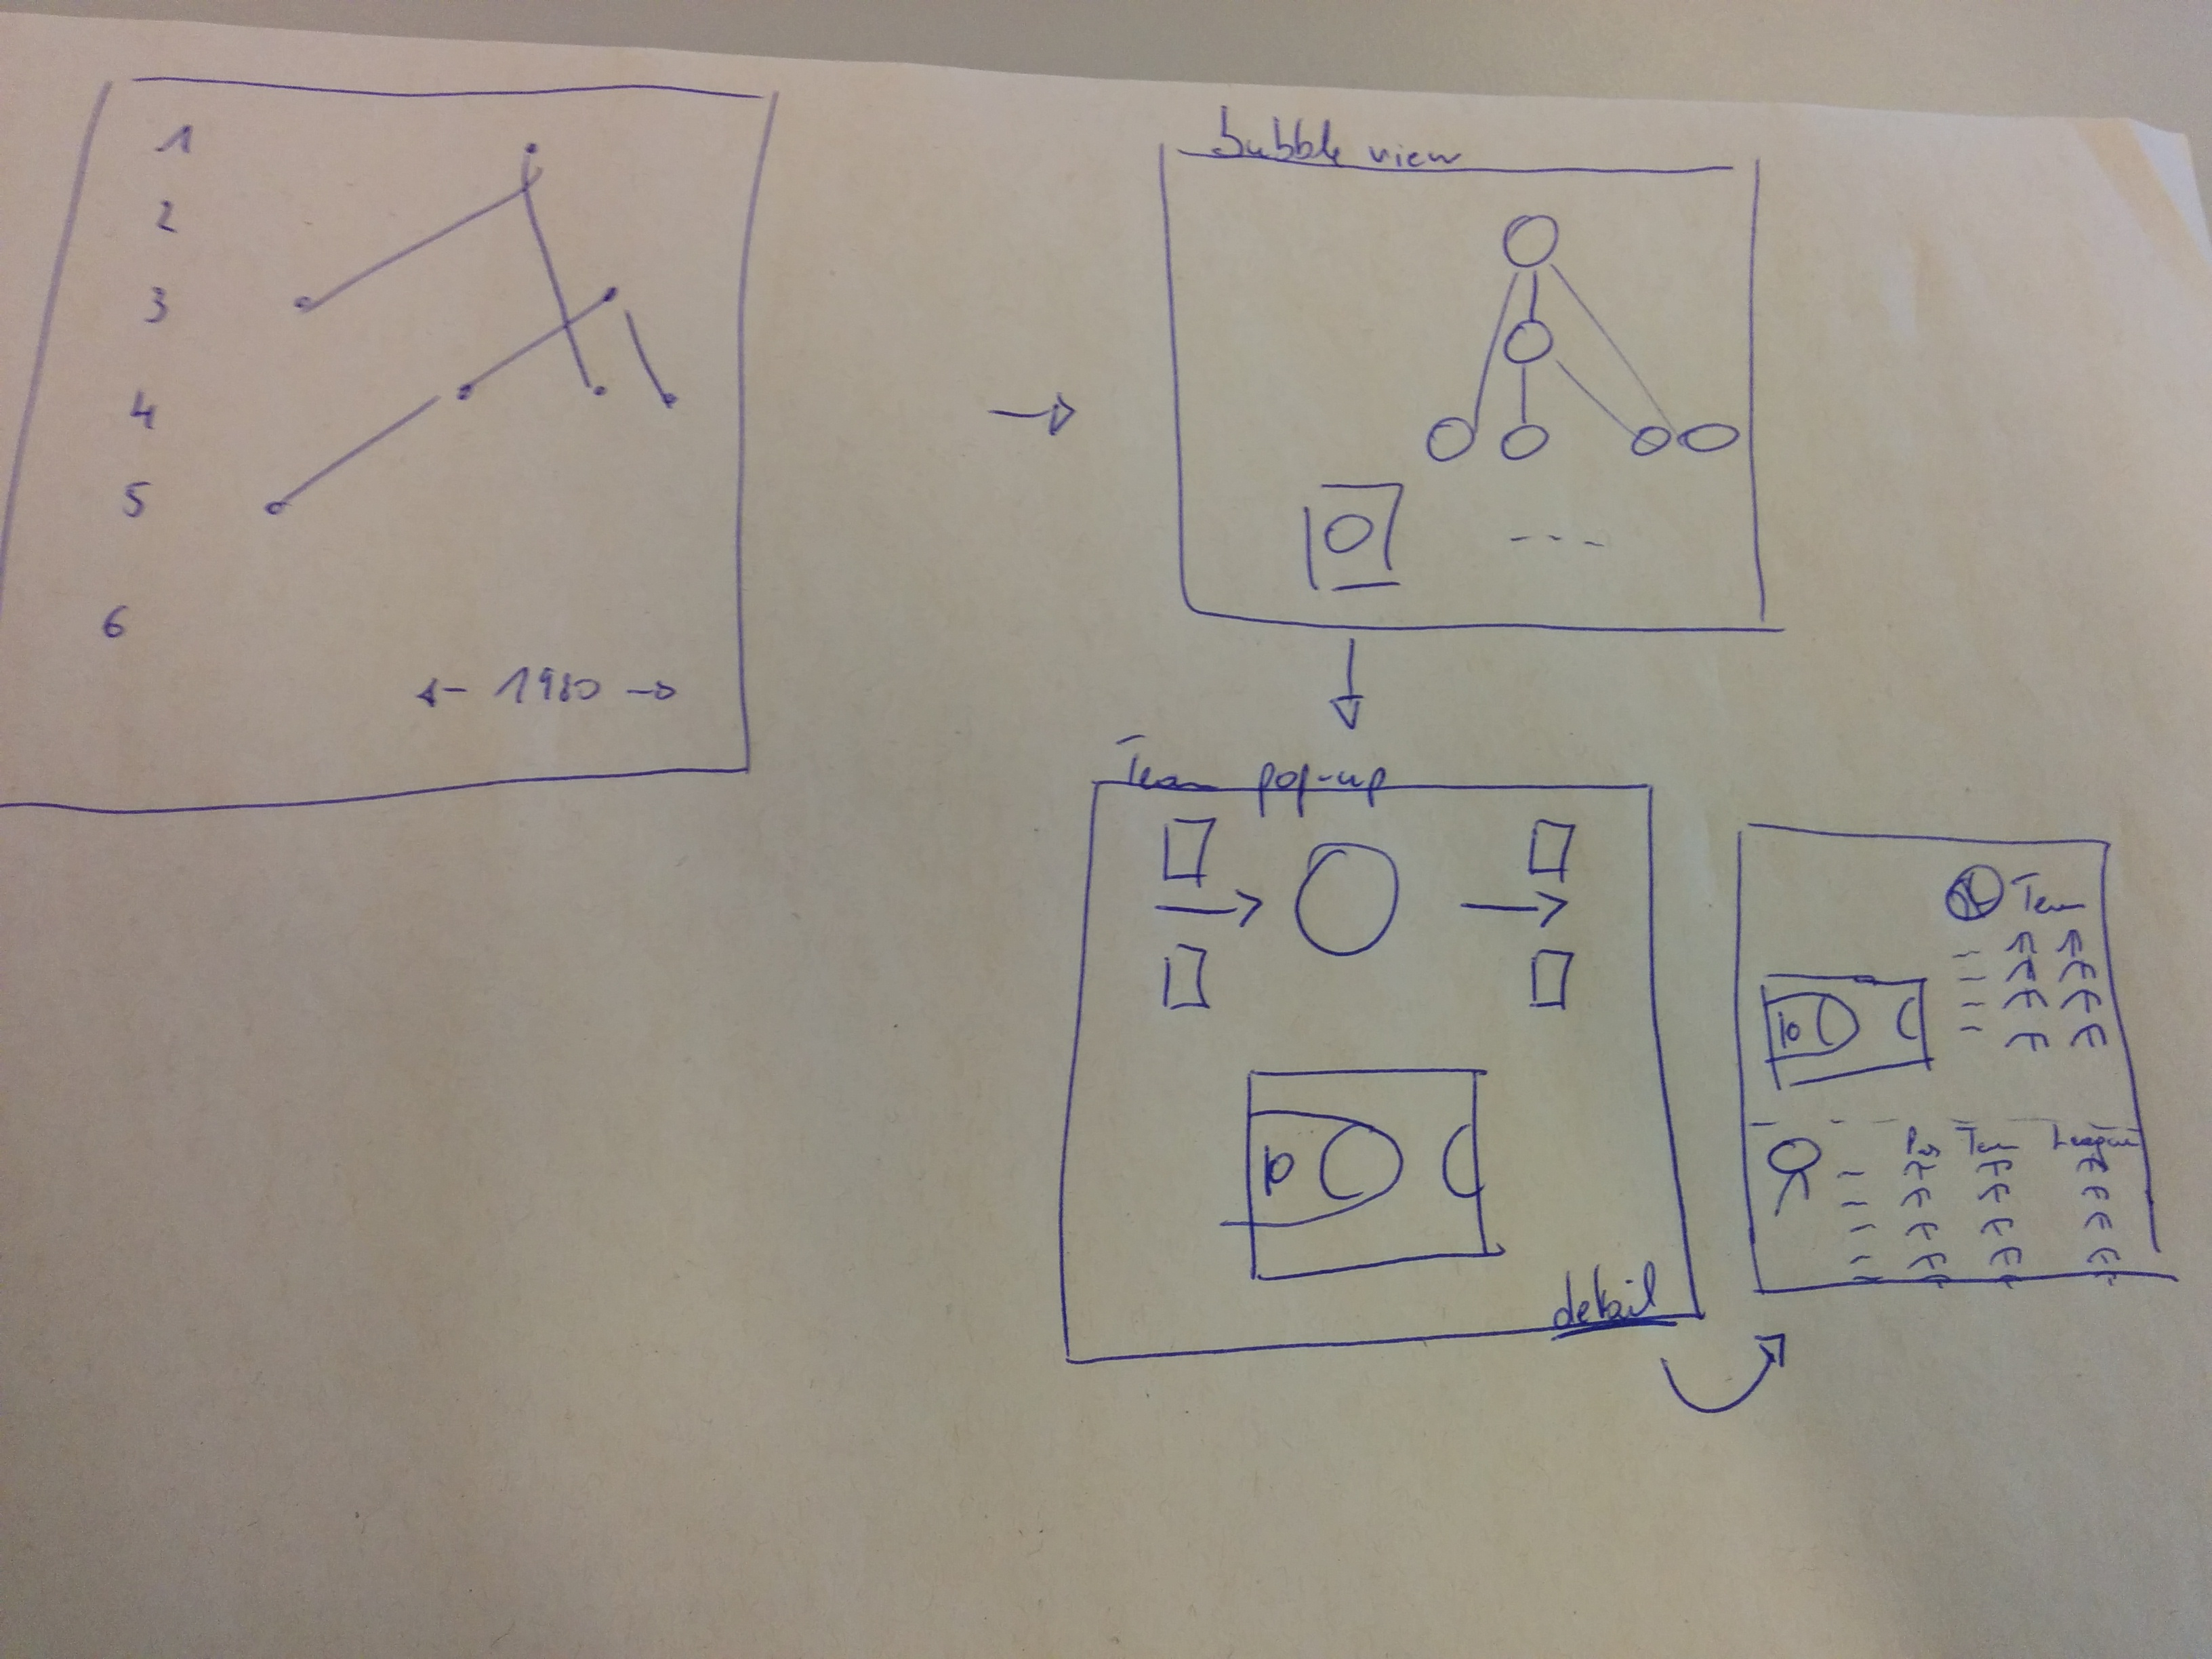
\includegraphics[width=1.0\columnwidth]{figures/smallmultsketch}
  \caption{A sketch of a previous design including the small multiples on the
  bottom right.}
  \label{fig:smallmultsktech}
\end{figure}

\subsection{Technology}
To create the visualization, the d3 javascript framework~\cite{d3} was used in
combination with html5~\cite{html5} and jquery~\cite{jquery}. Note that D3 is
based on HTML, CSS, Javascript and SVG. This allows easy access to the
visualization as most modern browsers are capable of handling these
webstandards. The choice not to use the d3 framework for the entire
visualization was made to ease the layout configuration of the visualization.
Instead, html was used to do the global layout of the visualization. We opted to
structure the site with multiple divs as containers. To each container we
allocate a svg with a specific visualization.
%\todo{sketch of how the page is structured here}

When working with d3.js we encountered one main obstacle:
\begin{itemize}
        \item A synchrounous call need to be combined with synchronous calls.
            More specific, when a visitor uses the timeline to scroll through
            time, the whiping of previous visualizations was not synced with the
            creation of the visualisation. This resulted in whiping sections
            when a visualization was not created yet. Hence the view resulted in
            multiple figures overlapping.
\end{itemize}


\section{Lessons learned}\label{sec:lessonslearned}
We've learned a couple of things during the creation of this visualization:
\begin{itemize}
    \item Find a story to tell with your visualization
    \item Each separate component should be a sufficient informative visualization on itself
    \item Creating a custom visualization costs time and opportunities
\end{itemize}
In what follows we will discuss our experience in more detail.

\subsection{Story telling}
At the beginning of this project we were able to design the 3 separate views
quite quickly. Our main concern was, when integrating these views as a whole, would 
we be able to see the relations and consequences we thought we would see and if 
we could draw the conclusions we hoped for. The relation we thought would be visible 
was that the total PER value of a team would influence the end positions in the NBA championship, both the league rank as the play-off rank. We expected that teams 
that had a big increase in total PER value, due to a good transferpolicy in a 
season, would benefit in one of the following seasons. It was not possible to draw this conclusion and according to us the reason for this is that a whole NBA team contains an average of 15 players. Some players may play a lot more than others and 
are therefore much more important to the team. This observation is why we could not draw our hoped conclusion, but at the same time we found it so interesting and we wondered if we could find an example to support this observation. The story is about 
the Chicago Bulls, the team of Michael Jordan who is seen as the greatest basketball 
player of all time. In 1984, Jordan arrives at the Chicago Bulls and in his first season he is already the top player of his team, as seen by the size of his jersey for the PER statistic. In the season 1990-1991 and the two following seasons, the 
Chicago Bulls win the NBA championship. The ``three-peat'' as it is called was done 
with almost the same core team. Next to Michael Jordan, there were around five 
players that were part of the team and were roughly the best on their position in 
the team, for example Scottie Pippen. We can see that in the seasons before this 
``three-peat'' this team was formed and already played with each other. After that 
last season form those three consecutive wins, Michael Jordan retires and the team 
is not able anymore to achieve the same. In the middle of the season 1994-1995, Michael Jordan came out of retirement. What follows is a similar story to the previous one. In the season 1995-1996 and the two following seasons, the Chicago 
Bulls again achieve to win the NBA chamionship three times in a row, again with a  team consisting of around five core players. Once again is Michael Jordan the star 
player of the team, but also Scottie Pippen is still one of the best players of the team. So to become the champion, it seems like a team needs to have a default team 
with around five core players and one or two star players.

%Our main problem was to integrate these views as a whole. When we
%created drafts of two views being the play-off view and the statitics view, we
%suddenly noted patterns. The Golden State Warriors became NBA champion a couple
%of years after a great uplift in SRS score. This was because of new players
%joining the team in 2009. In the years following, the team kept on attracting
%talented players and increased the inherent team score to become NBA champion in
%2015. With the team view, one can even notice that the team gets stronger in
%center team positions during this period. Users are able to explore the data for
%patters. On top of that, we provide the insight on how the changes were impacted
%by changes in teamplayers.

\subsection{Each component should be informative}
In order to have a good visualization as a whole, each component should be a
clear and informative visualization on itself. During the project, we started noticing that most components in a visualization lack references and hence are not informative enough. Eg. each small multiple of a statisctic in the statistics view on itself gives sufficient information to stand on itselfs. The bar in the small multiple indicates the score in the selected season and enables the user to evaluate that score over time. Have there been better scores, or worse scores. Is this score
part of an upward movement during years? This should be weighed against the
duplication of data and use of screen space. Coordinated views alleviate this
need significantly as well, as each component is strongly supported by other
components.

\subsection{Custom visualizations}
Before exploring what is out there in the d3.js world, we made our own sketches.
This is how we came up with the 3 custom views that make up our visualization.
When comparing our design with alternatives we could not find something that
satisfied our needs. Nonetheless, they gave us inspiration to finetune our
designs. Although we are satisfied with our result and we are convinced it was
the right choice to reach our goal, it had some draw backs. If we would have not started with our custom view, we would have had more freedom in exploring multiple different visualizations and we would be able to evaluate different options with trial and error. Instead much of the time developing was spent on the technical details for these custom visualizations. This was especially true for the bubble component of the play-off view. No out of the box solution for this could be found so everything from the determination of the positions of the bubbles to how to connect them had to be developed by us.

\section{Future work}\label{sec:futurework}
As with most projects, the result is never 'finished', meaning that there are
always extensions and iprovements possible but due to timing or resource constraints they haven't all been implemented. We suggest a number of features that might improve the visualization:
\begin{itemize}
    \item Smooth transitions between states could improve the user experience.
        For example when changing year, a transformation of the arrow in the
        statistics view would help the user see a difference between years.  At
        the moment the arrows change at the blink of an eye, making it difficult
        for us humans with a short term memory to make the comparison. This
        would also have been very useful in the transitions between different
        years on the bubble view.
    \item To further support our short term memory we could also 'save' the
        previous state. Eg. in the field view we could visualize ghost jerseys
        to indicate which players left the team or position and highlight
        players that joined the team.  This would help the user see how the team
        changes over time.
    \item At the moment no attention has been payed to the process, provenance
        and history of the user's exploration session. A user thus needs to
        memorize his action to be able to share or reproduce his actions. This
        could be improved by adding URL parameters. This way a user at least can
        share or save a state of an analysis. One step further is to provide a
        play-feature. The visitor could them share his exploration and replay
        it. A simple implemention would ask the visitor for a start date and an
        end date and would then 'play' the changes of a particular team and
        characteristic over time.
    \item We could support users further in looking for patterns by focussing
        more on comparisons. We could integrate a view where a visitor is able
        to compare two teams in the same year, or in two different years.
    \item We could focus more on the core team, i.e. five or six players who seems 
        to be the most important for the results of a team.
\end{itemize}

\section{Conclusion}\label{sec:conclusion}
We believe the visualization we have created can be of tremendous value for fans
and fantasy basketball players. Personally we have gained several insights into
the performance of basketball teams by using the visualization and we believe
others could learn even more. 
The most interesting conclusion we were able to make concerns the importance of
individual players in a basketball team. We were able to find strong
correlations between having two to four very strong players and the team's
performance. It seems having one star player is not enough. On the other hand,
having more than 5 good players no longer has much influence either. 

While the visualization has a lot of potential for improvement, we think the
innovative play-offs representation combined with detailed team information in
an integrated fashion has much value.

% Balancing columns in a ref list is a bit of a pain because you
% either use a hack like flushend or balance, or manually insert
% a column break.  http://www.tex.ac.uk/cgi-bin/texfaq2html?label=balance
% multicols doesn't work because we're already in two-column mode,
% and flushend isn't awesome, so I choose balance.  See this
% for more info: http://cs.brown.edu/system/software/latex/doc/balance.pdf
%
% Note that in a perfect world balance wants to be in the first
% column of the last page.
%
% If balance doesn't work for you, you can remove that and
% hard-code a column break into the bbl file right before you
% submit:
%
% http://stackoverflow.com/questions/2149854/how-to-manually-equalize-columns-
% in-an-ieee-paper-if-using-bibtex
%
% Or, just remove \balance and give up on balancing the last page.
%
\balance{}

% REFERENCES FORMAT
% References must be the same font size as other body text.
%\bibliographystyle{SIGCHI-Reference-Format}

\printbibliography

\appendix
\section{Terminology}\label{sec:terminology}

\paragraph{NBA} National Basketball Association - The largest, most well-known
basketball of the USA.

\paragraph{PER} Player Efficiency Rating - An all-in-one basketball rating,
boiling down all of a player's contributions into one number\cite{per}.

\paragraph{SRS} Simple Rating System - a rating that takes into account average
point differential and strength of schedule. The rating is denominated in points
above/below average, where zero is average\cite{srs}. 

\paragraph{Playoffs} The National Basketball Association (NBA) playoffs are a
best-of-seven elimination tournament among 16 teams in the Eastern Conference
and Western Conference (called divisions, pre-1970), ultimately deciding the
winner of the NBA Finals\cite{playoffs}.

\paragraph{Jersey} The shirt worn by basketball players.


\end{document}

%%% Local Variables:
%%% mode: latex
%%% TeX-master: t
%%% End:
